% Chapter Template

\chapter{Ensayos y resultados} % Main chapter title



\label{Chapter4} % Change X to a consecutive number; for referencing this chapter elsewhere, use \ref{ChapterX}

En este capítulo se presentan y describen los ensayos llevados a cabo y las técnicas implementadas para verificar la funcionalidad de cada componente desarrollado y del sistema en su totalidad. Además, se muestran y analizan los resultados obtenidos en cada prueba.

%----------------------------------------------------------------------------------------
%	SECTION 1
%----------------------------------------------------------------------------------------

\section{Banco de pruebas}

El banco de pruebas que se utilizó para este trabajo, estuvo conformado por los elementos descritos en la tabla \ref{tab:banco-pruebas}:

\begin{table}[H]
	\centering
	\caption{Banco de pruebas.}
	\begin{tabular}{l c c}    
		\toprule
		\textbf{Elemento} 	 & \textbf{Aplicación} \\
		\midrule
		Computadora local & Despliegue local de \textit{frontend} y \textit{backend}.  \\		
		Prototipo de hardware & Botón antipánico. \\		
		Chip GSM & \makecell{Número de teléfono para el envío de  SMS en el \\ hardware.} \\
		Postman & Herramienta para pruebas manuales del \textit{backend}.\\
		Número de Twilio & \makecell{Número de teléfono virtual para la recepción \\ de SMS.}  \\
		Multímetro & Herramienta para medir consumo energético.  \\
		CP2102 & \makecell{Conversor de puerto serie a USB \\ para \textit{debugging} \citep{CP2102:1}.}\\	
		\bottomrule
		\hline
	\end{tabular}
	\label{tab:banco-pruebas}
\end{table}

En relación a las pruebas a realizar para verificar el cumplimiento de los componentes desarrollados, se determinaron las siguientes:

\begin{itemize}
\item Dispositivo embebido:
	\begin{itemize}
	\item Prueba de almacenamiento de las latitud, longitud, IMEI, teléfono almacenado.
	\item Prueba de SMS de configuración de teléfono.
	\item Medición de consumo energético de módulos de hardware.
	\item Prueba de medición de carga de batería.
	\item Prueba de pulsación de botón de alerta y envío de SMS con datos de localización.
	\end{itemize}
\item \textit{Backend}:
	\begin{itemize}
	\item Prueba de creación de usuario administrador y su organización.
	\item Prueba de obtención/creación/modificación/desactivación de beneficiarios.
	\item Prueba de obtención/creación/modificación/desactivación de tipos de beneficiarios.
	\item Prueba de obtención/creación/modificación/desactivación de tipos de alertas.
	\item Prueba de obtención/actualización de alertas.
	\item Prueba de conexión a canal de \textit{WebSockets}.
	\item Prueba de recepción de alerta mediante \textit{webhook}.
	\item Prueba de bloqueo de nueva alerta para un número de teléfono no habilitado.
	\end{itemize}
\item \textit{Frontend}:
	\begin{itemize}
	\item Prueba de registro.
	\item Prueba de \textit{login}.
	\item Prueba de visualización de últimas alertas recibidas.
	\item Prueba de atención de nuevas alertas.
	\item Prueba de recepción de nuevas alertas en tiempo real.
	\item Prueba de visualización/modificación/creación/eliminación de beneficiarios, tipos de beneficiarios y tipos de alerta.
	\item Prueba de visualización y exportación de alertas.
	\end{itemize}

\end{itemize}


\section{Metodología empleada}

Para poder ver los mensajes informativos del firmware, al momento de hacer pruebas, se conectó la salida del puerto UART0 del ESP32 como se observa en la figura \ref{fig:cp2102}, usado para mensajes de \textit{debug} por parte del ESP32 \citep{UART:1}, al dispositivo CP2102 que permite enviar los mensajes al puerto USB de la computadora.

\begin{figure}[H]
	\centering
    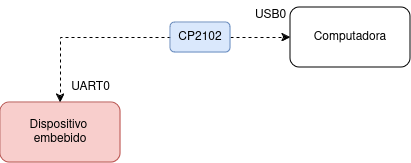
\includegraphics[width=0.6\linewidth]{./Figures/cp2102.png}
    \captionof{figure}{Esquema de conexión del CP2102.}
    \label{fig:cp2102}
\end{figure}

En la figura \ref{fig:esp32:debug} se observan mensajes enviados por puerto serie. Esto es porque en las pruebas integrales, no se utilizó la alimentación por USB del ESP32, sino que se utilizó la batería, perdiendo la posibilidad de ver directamente la salida del ESP32.

\begin{figure}[H]
	\centering
    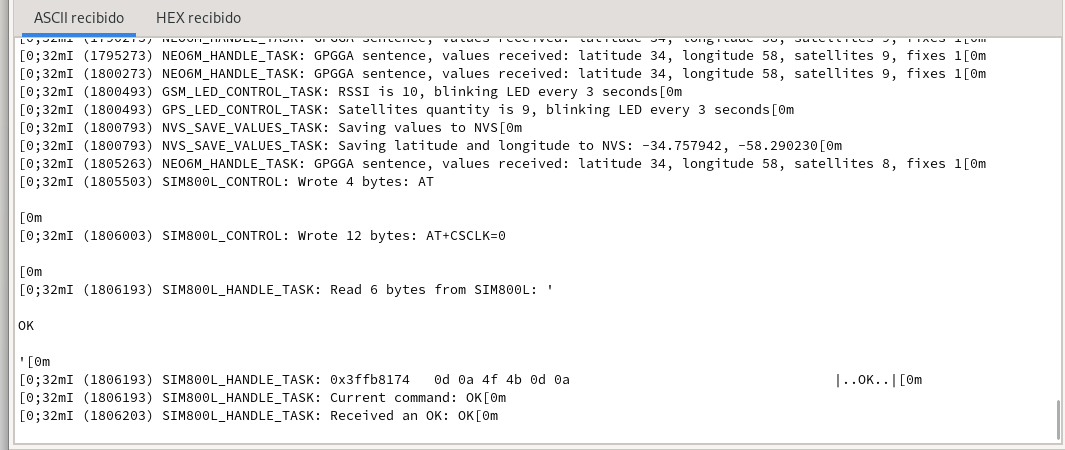
\includegraphics[width=0.95\linewidth]{./Figures/moserial-debug.png}
    \captionof{figure}{Salida del ESP32 vista en Moserial.}
    \label{fig:esp32:debug}
\end{figure}


Para medir el consumo energético, se configuró el multímetro con la disposición observada en la figura \ref{fig:pruebas:multimetro}, es decir, en serie con los módulos de hardware:

\begin{figure}[H]
	\centering
	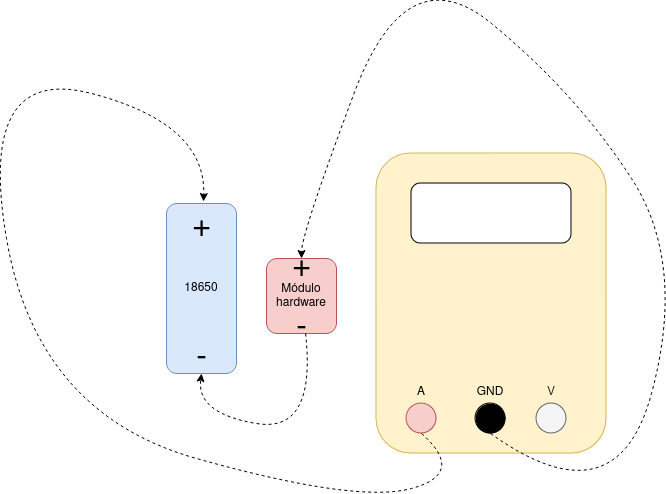
\includegraphics[width=0.9\textwidth]{./Figures/multimetro.png}
	\caption{Esquema de conexión del multímetro.}
	\label{fig:pruebas:multimetro}
\end{figure}

Además, se contrastó en las mediciones el consumo informado por el \textit{datasheet} del fabricante de cada módulo, para determinar si efectivamente las mediciones fueron correctas. Se concluyó de que la calidad de las mediciones eran aceptables, aunque lo ideal hubiese sido contar con un osciloscopio. Por otra parte, las pruebas de consumo energético se realizaron primero de forma aislada con cada componente y luego se midió el consumo total del dispositivo embebido. 

Es importante destacar la necesidad de desplegar la aplicación en un entorno \textit{cloud} para las pruebas, ya que la integración con Twilio no fue posible con la instalación local. La base de datos local se configuró utilizando una imagen Docker con PostgreSQL \citep{DOCKER:2}.

Para verificar el funcionamiento del sistema web se implementó una cantidad de pruebas unitarias en el \textit{backend} con la biblioteca \textit{APITestCase}, provista por el framework Django para el desarrollo de pruebas unitarias \citep{DJANGO:13}. Estas pruebas permitieron validar que la API funcionase correctamente para las operaciones básicas.

Por otra parte, se realizaron algunas pruebas de forma manual mediante el uso de Postman, herramienta para desarrollo y testing de APIs para algunos casos particulares, como:
\begin{itemize}
	\item Establecimiento de conexión mediante \textit{WebSockets}.
	\item Verificación de recepción de nuevas alertas en tiempo real mediante el canal de \textit{WebSockets}.
\end{itemize}

Para verificar el funcionamiento correcto del \textit{frontend}, se realizaron pruebas conectadas con el \textit{backend}.

\section{Pruebas de módulos de hardware}

En la figura \ref{fig:esp32:fisico} se puede visualizar la disposición física del dispositivo embebido.
\begin{figure}[H]
	\centering
	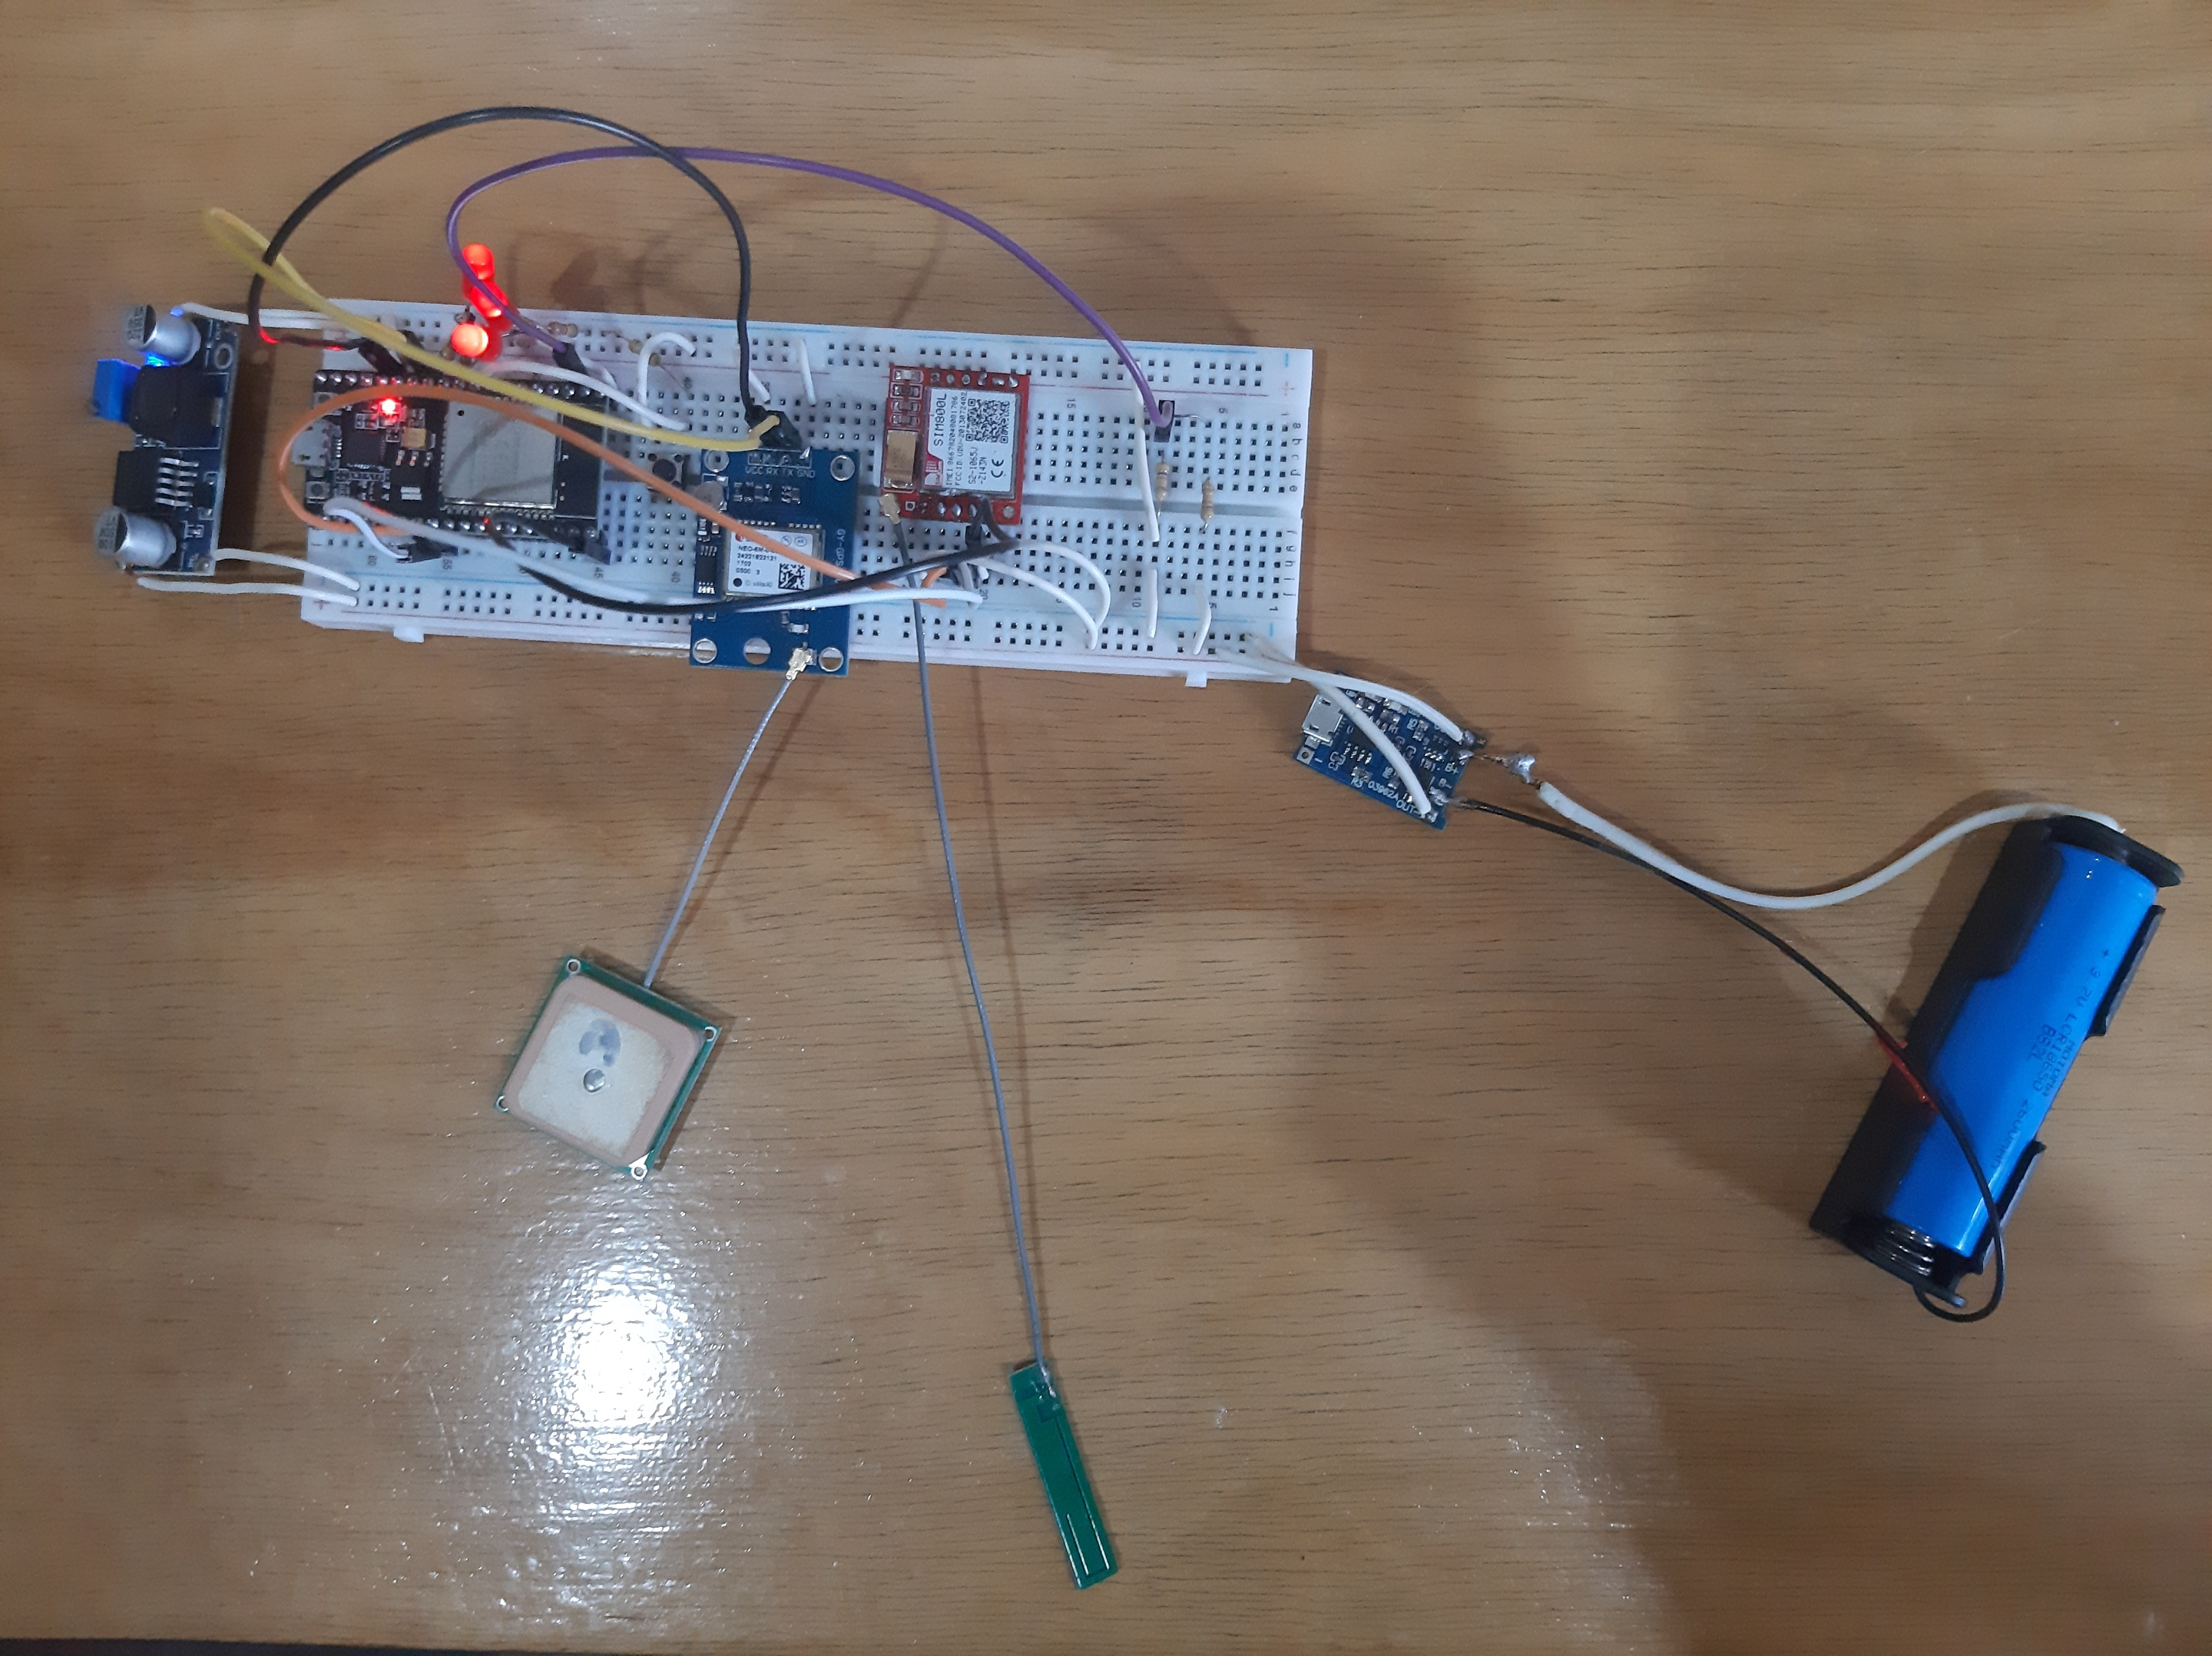
\includegraphics[width=1\textwidth]{./Figures/esp32-fisico.jpg}
	\caption{Esquema de componentes de hardware del ESP32.}
	\label{fig:esp32:fisico}
\end{figure}

Respecto al almacenamiento de variables, la figura \ref{fig:esp32:nvs} muestra la lectura de variables almacenadas.

\begin{figure}[H]
	\centering
	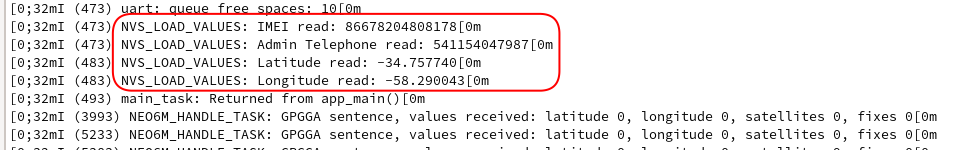
\includegraphics[width=1\textwidth]{./Figures/esp32-nvs.png}
	\caption{Lectura de variables almacenadas en el almacenamiento no volátil.}
	\label{fig:esp32:nvs}
\end{figure}

De todas maneras, se encontraron inconvenientes esporádicos con las variables de latitud y longitud almacenadas, ya que cada ciertos reinicios o reinstalación del firmware, las variables en el almacenamiento no volátil se reinicializaban.

Posteriormente, se chequeó la recepción del SMS de configuración de número telefónico de Twilio que incluye parte del IMEI del dispositivo como validación, como se puede visualizar en la figura \ref{fig:esp32:sos}. En esta prueba, el mensaje que se envió fue \texttt{sos866782 0014254096083}.

\begin{figure}[H]
	\centering
	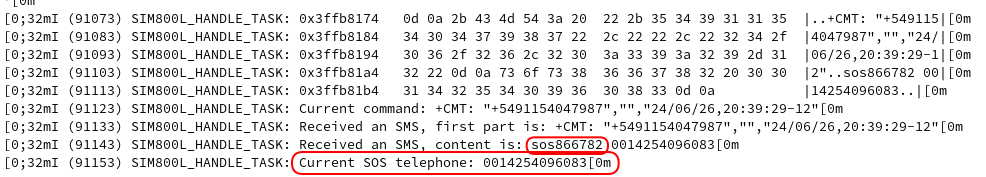
\includegraphics[width=1\textwidth]{./Figures/esp32-sos.png}
	\caption{Configuración de número telefónico para la recepción de alertas.}
	\label{fig:esp32:sos}
\end{figure}


En la tabla \ref{tab:pruebas:energia} se puede observar el listado de consumo energético medido.

\begin{table}[H]
	\centering
	\caption[Mediciones de consumo energético.]{Mediciones de consumo energético.}
	\begin{tabular}{l c c c}    
		\toprule
		\textbf{Elemento} 	 & \textbf{\makecell{Consumo \\ base}} & \textbf{\makecell{Consumo optimizado \\ según \textit{datasheet} }} & \textbf{\makecell{Consumo optimizado \\ según pruebas}}  \\
		\midrule
		ESP32 & 30 $\sim$ 68 mA \citep{ESP32:1} & 20 mA \citep{ESP32:1} & 16 mA \\		
		LM2596 & 20 mA \citep{LM2596:1} & 5 mA &  12 mA \\	
		NEO-6M & 41 mA \citep{NEO6M:2} & 8 mA & 11 $\sim$ 30 mA \\	
		SIM800L & 60 mA \citep{SIM800L:1} & $<$ 7 mA & 10 $\sim$ 40 mA \\		
		\bottomrule
		\textbf{Total} & 140 mA & 40 mA & 49 $\sim$ 98 mA \\
		\bottomrule
		\hline
	\end{tabular}
	\label{tab:pruebas:energia}
\end{table}

Para las mediciones no se contabilizaron pequeños componentes como LEDs y resistencias ya que su consumo total, alrededor de 1 mA, representa un porcentaje despreciable del consumo completo.

Por otra parte, las mediciones son promedios, no picos de consumo debido a las limitaciones del multímetro de bajo costo utilizado. De todas maneras, se pudo validar el consumo indicado por los \textit{datasheets} de los módulos, aunque se encontraron diferencias al realizar mediciones posteriores a las optimizaciones de energía. Se obsevaron grandes diferencias entre mínimos y máximos de los módulos NEO-6M y SIM800L y esto es debido a que cuando los módulos e inicializan tienen un promedio de consumo alto, siendo estabilizado el consumo transcurrido un tiempo. Para concluir, se promedió el consumo del prototipo en 60 mA, lo que resultó en un aproximado de más de 30 horas de autonomía en condiciones ideales y suponiendo que la batería asignada efectivamente tiene la capacidad indicada. Si bien este valor no alcanza a los objetivos iniciales, significa una duración aceptable en comparación a otros modelos de dispositivos.


El cálculo de carga de la batería se realizó mediante una aproximación lineal, siendo el voltaje medido una referencia de la carga real de la batería. En la figura \ref{fig:esp32:bateria} se observa el valor calculado en una de las pruebas.

\begin{figure}[H]
	\centering
	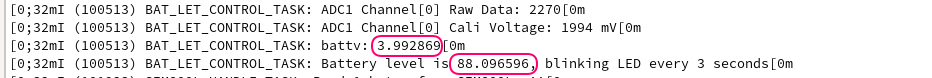
\includegraphics[width=1\textwidth]{./Figures/esp32-battery.png}
	\caption{Cálculo de carga de batería.}
	\label{fig:esp32:bateria}
\end{figure}

Por último, se puede visualizar en la figura \ref{fig:esp32:alerta} el disparo de una alerta y el envío del SMS con el contenido de la localización.

\begin{figure}[H]
	\centering
	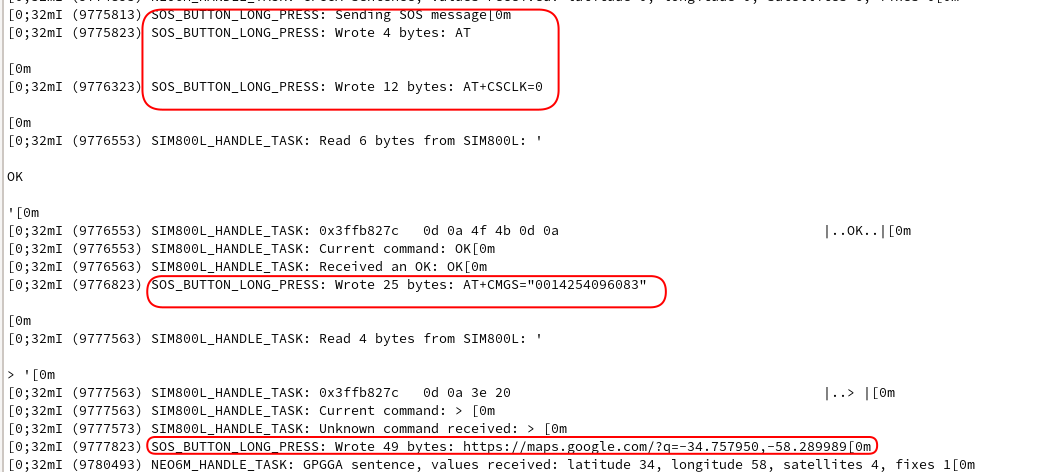
\includegraphics[width=1\textwidth]{./Figures/esp32-alerta.png}
	\caption{Disparo de alerta desde el dispositivo embebido.}
	\label{fig:esp32:alerta}
\end{figure}

\subsection{Pruebas adicionales}

Debido a que se detectaron mediciones elevadas en el ESP32 incluso durante la aplicación de \textit{light sleep}, se realizaron pruebas adicionales con otra placa de desarrollo, ESP32-C3, cuyas prestaciones son ligeramente diferentes \citep{ESP32C3:1}. Con este dispositivo se probó solamente el firmware adaptado, sin los módulos externos y se verificó que efectivamente el consumo era aproximadamente 1 mA. Esto permitió concluir que el kit ESP32-WROOM-32 de NodeMCU no está preparado para configuraciones de bajo consumo. 
De todas maneras, no se avanzó en la re-implementación del firmware debido a que implicaba acomodar varias configuraciones adicionales como el uso de puertos serie, pines en uso, entre otros. En caso de haber continuado con la implementación del modo \textit{light sleep} de forma automática, hubiera sido necesario volver a realizar pruebas con todos los módulos. La ventaja de utilizar el modo automático de \textit{light sleep} es que gran parte del tiempo \textit{idle} del ESP32 hubiera representado un ahorro de energía de varios mA.

Por otra parte, se intentó reemplazar el regulador de tensión LM2596 por el regulador de tensión lineal LD1117 cuyo consumo en es menor \citep{LD1117:1}, pero el \textit{dropout} de voltaje resultó muy elevado para el ESP32 y el NEO-6M, al punto de no ser suficiente para que funcionen correctamente.

\section{Pruebas de sistema web}

En esta sección se presentan las pruebas implementadas para los componentes del sistema web, diferenciadas por las pruebas a nivel API y las pruebas a nivel aplicación usuario.

\subsection{Pruebas de \textit{backend}}

La figura \ref{fig:tests-unitarios} muestra la ejecución correcta de los 24 tests unitarios desarrollados con la biblioteca \textit{APITestCase} de \textit{backend}:

\begin{figure}[H]
	\centering
	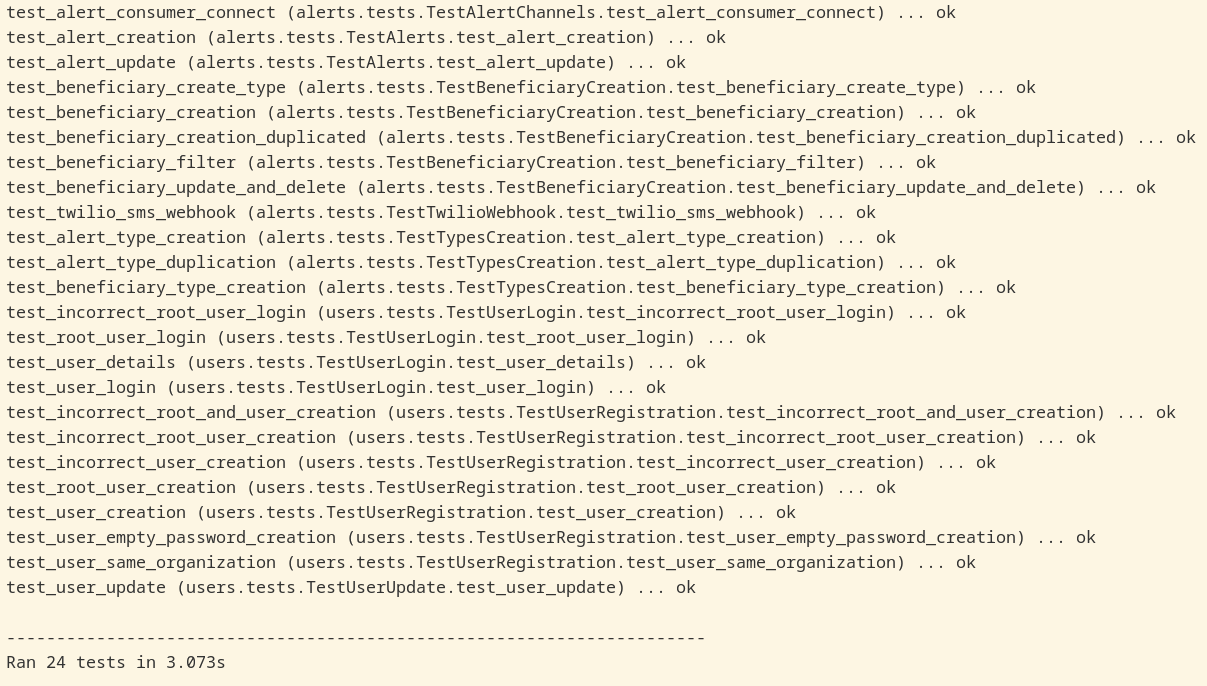
\includegraphics[width=1\textwidth]{./Figures/tests-unitarios.png}
	\caption{Ejecución correcta de tests unitarios del \textit{backend}.}
	\label{fig:tests-unitarios}
\end{figure}

De todas maneras, se realizaron algunas pruebas manuales adicionales debido a casos de uso no contemplados originalmente, como actualizaciones parciales sobre entidades. Para el caso de la conexión a \textit{WebSockets}, se muestran en las figuras \ref{fig:postman1} y \ref{fig:postman2} las pruebas hechas de forma manual mediante Postman para la conexión al canal de comunicación en tiempo real y la recepción de una nueva alerta. 

\begin{figure}[H]
	\centering
  	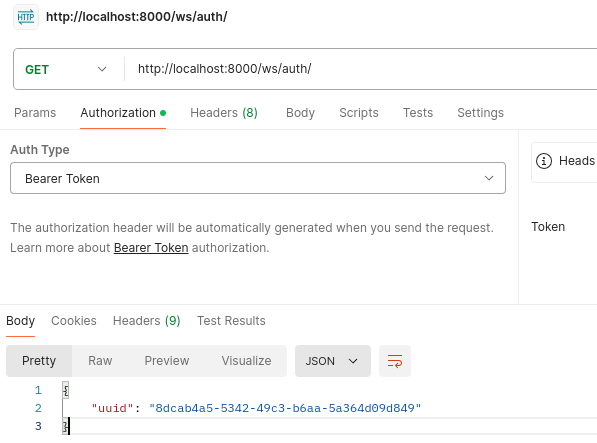
\includegraphics[width=0.9\linewidth]{./Figures/postman1.png}
  	\captionof{figure}{Obtención de un token efímero para \textit{WebSockets}.}
  	\label{fig:postman1}
\end{figure}

En el caso de la figura \ref{fig:postman2} se puede apreciar la marca de tiempo cuando se estableció la conexión y más tarde se recibió publicada la nueva alerta.

\begin{figure}[H]
	\centering
  	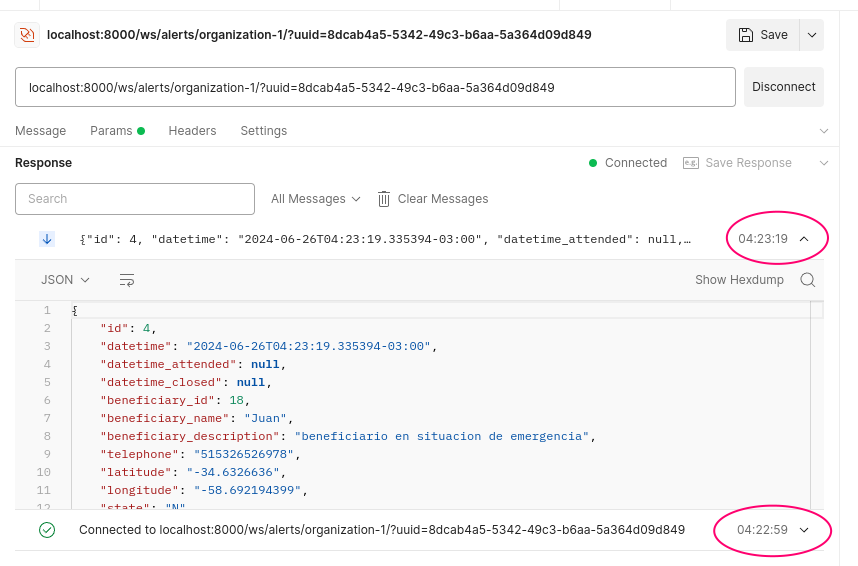
\includegraphics[width=1\linewidth]{./Figures/postman2.png}
  	\captionof{figure}{Conexión a \textit{WebSockets} y recepción de una nueva alerta.}
  	\label{fig:postman2}
\end{figure}

Para la recepción de alertas de Twilio, se verificó la generación de una alerta mediante el envío de un SMS al número telefónico de Twilio. En la figura \ref{fig:backend-twilio} se puede apreciar la respuesta del \textit{backend} cuando Twilio invoca el \textit{webhook} con los datos de un número telefónico desconocido. Para probar localmente este \textit{endpoint}, se desactivó la validación de credenciales de Twilio.

\begin{figure}[H]
	\centering
  	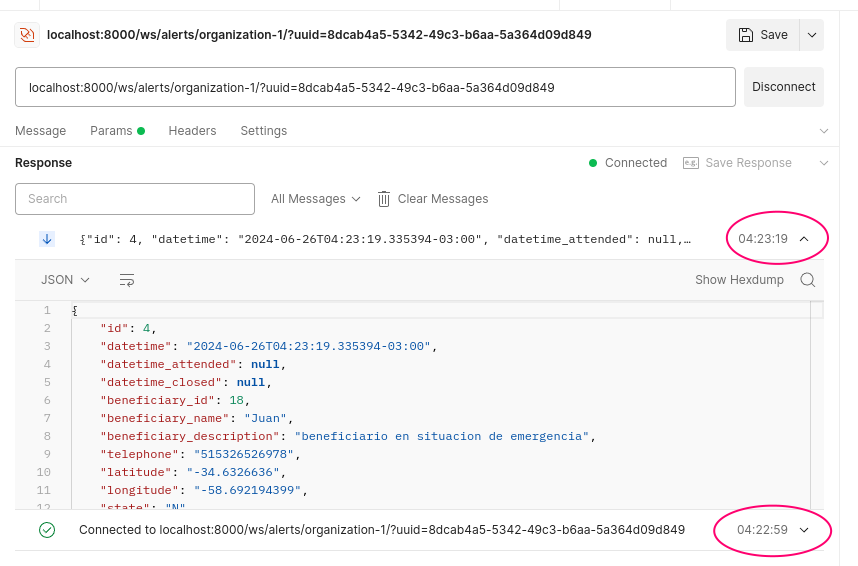
\includegraphics[width=1\linewidth]{./Figures/postman2.png}
  	\captionof{figure}{Validación de beneficiario existente al momento de generar una alerta.}
  	\label{fig:backend-twilio}
\end{figure}

\subsection{Pruebas de \textit{frontend}}

Para poder verificar todos los requerimientos del \textit{frontend} listados en el banco de pruebas, se llevaron a cabo pruebas manuales sobre todas las secciones desarrolladas. En las figuras \ref{frontend:registro} y \ref{frontend:login} se pueden apreciar las pantallas de registro e ingreso.


\begin{figure}[H]
\centering
\begin{minipage}{.5\textwidth}
  \centering
  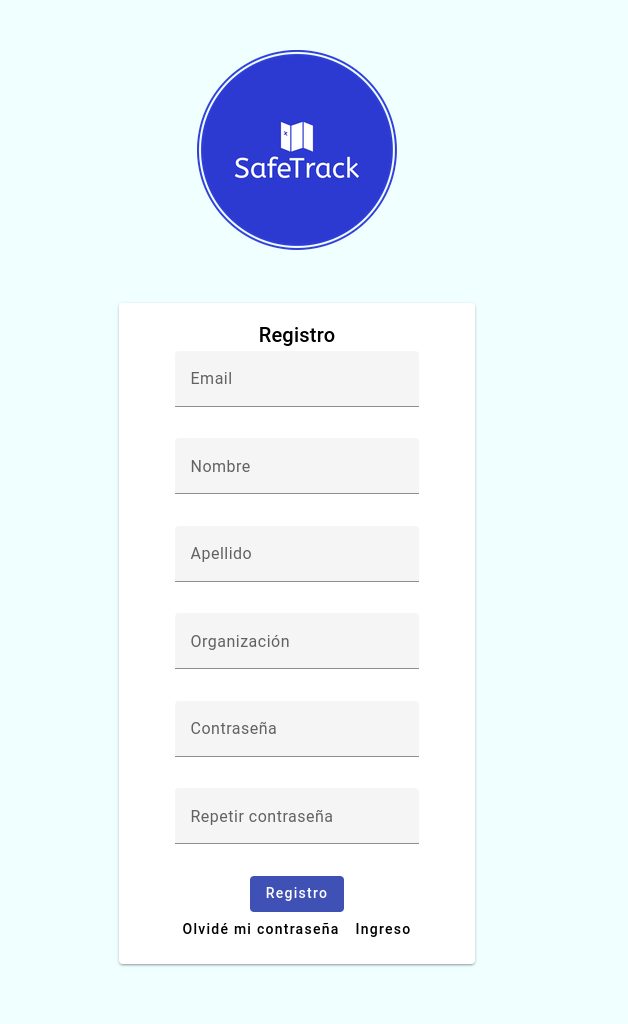
\includegraphics[width=0.9\linewidth]{./Figures/registro.png}
  \captionof{figure}{Pantalla de registro.}
  \label{frontend:registro}
\end{minipage}%
\begin{minipage}{.5\textwidth}
  \centering
  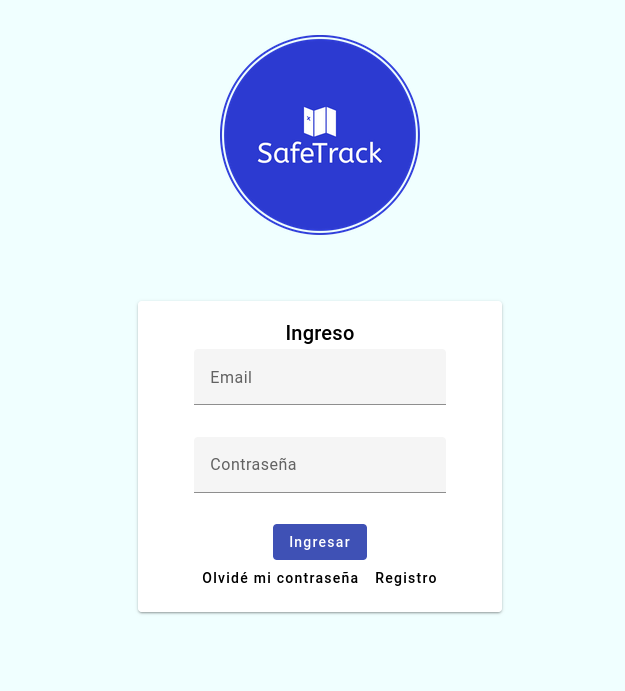
\includegraphics[width=0.9\linewidth]{./Figures/login.png}
  \captionof{figure}{Pantalla de ingreso.}
  \label{frontend:login}
\end{minipage}
\end{figure}


En relación a la visualización y atención de alertas en tiempo real, se implementó la sección de mapa con el listado de alertas recientes a la izquierda. En la figura \ref{fig:frontend:mapa} se puede observar una alerta generada desde el botón antipánico directamente.

\begin{figure}[H]
	\centering
  	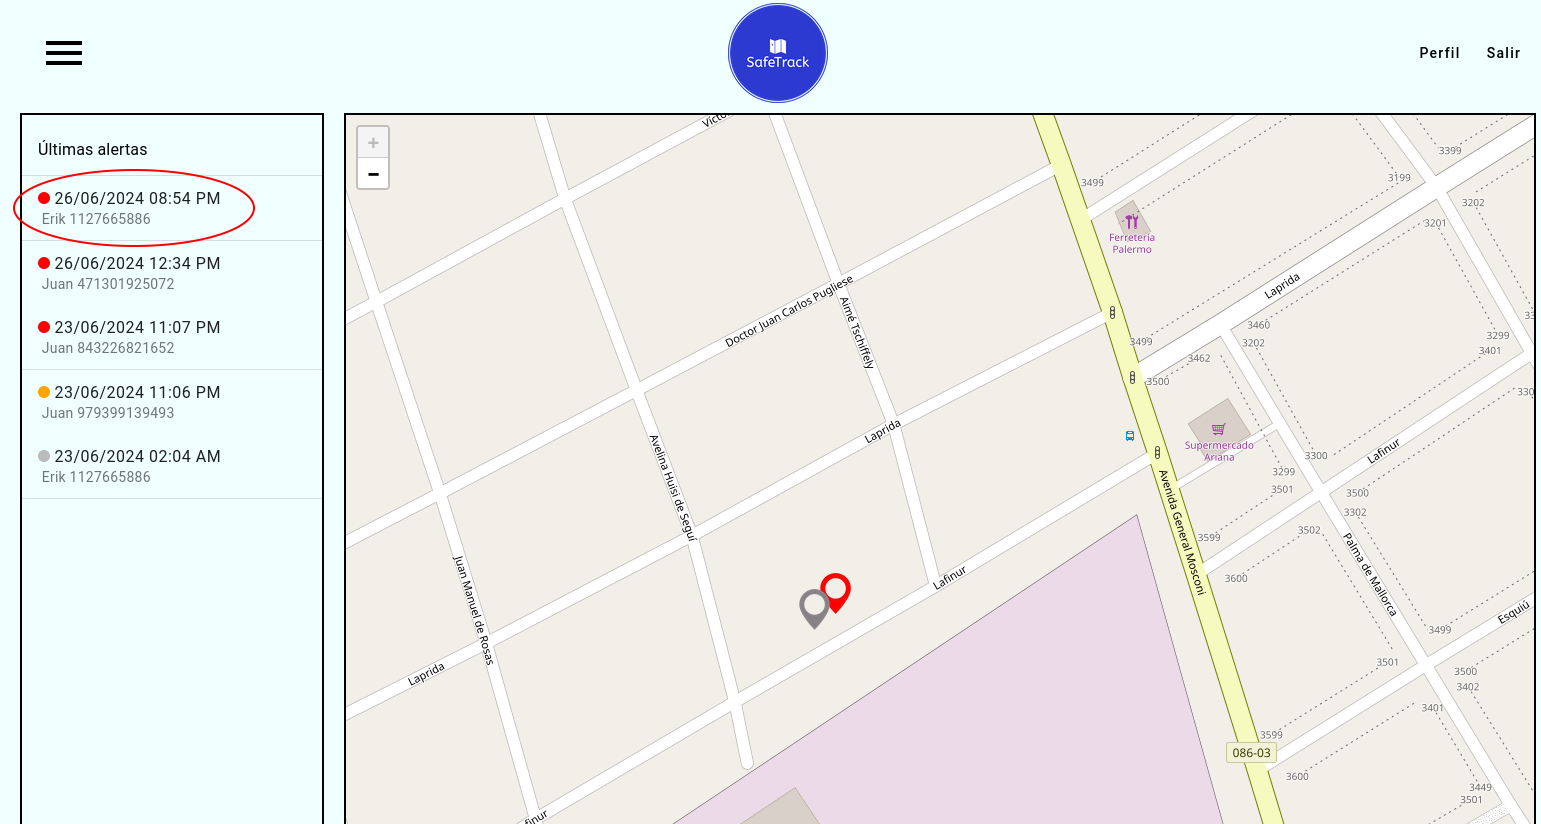
\includegraphics[width=1\linewidth]{./Figures/frontend-alerta.png}
  	\captionof{figure}{Mapa con alertas.}
  	\label{fig:frontend:mapa}
\end{figure}	
	
Por otra parte se probaron los tres menús de carga creados, beneficiarios, tipos de beneficiarios y tipos de alertas, y se pudo visualizar la sección de beneficiarios en la figura \ref{fig:frontend:beneficiarios} con algunos datos creados.

\begin{figure}[H]
	\centering
  	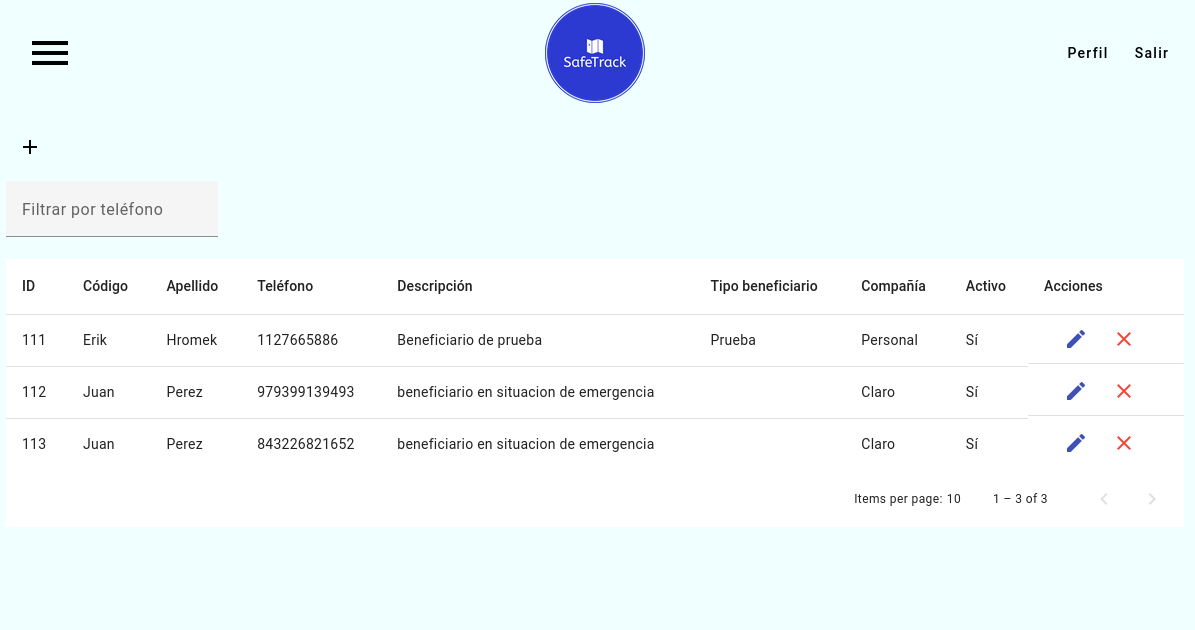
\includegraphics[width=1\linewidth]{./Figures/listado-beneficiarios.png}
  	\captionof{figure}{ABM de beneficiarios.}
  	\label{fig:frontend:beneficiarios}
\end{figure}
	
Además, se implementó una sección para visualizar el historial de alertas y poder exportarlo a un archivo de extensión CSV mediante un botón, como se verifica en la figura \ref{fig:frontend:alertas}.

\begin{figure}[H]
	\centering
  	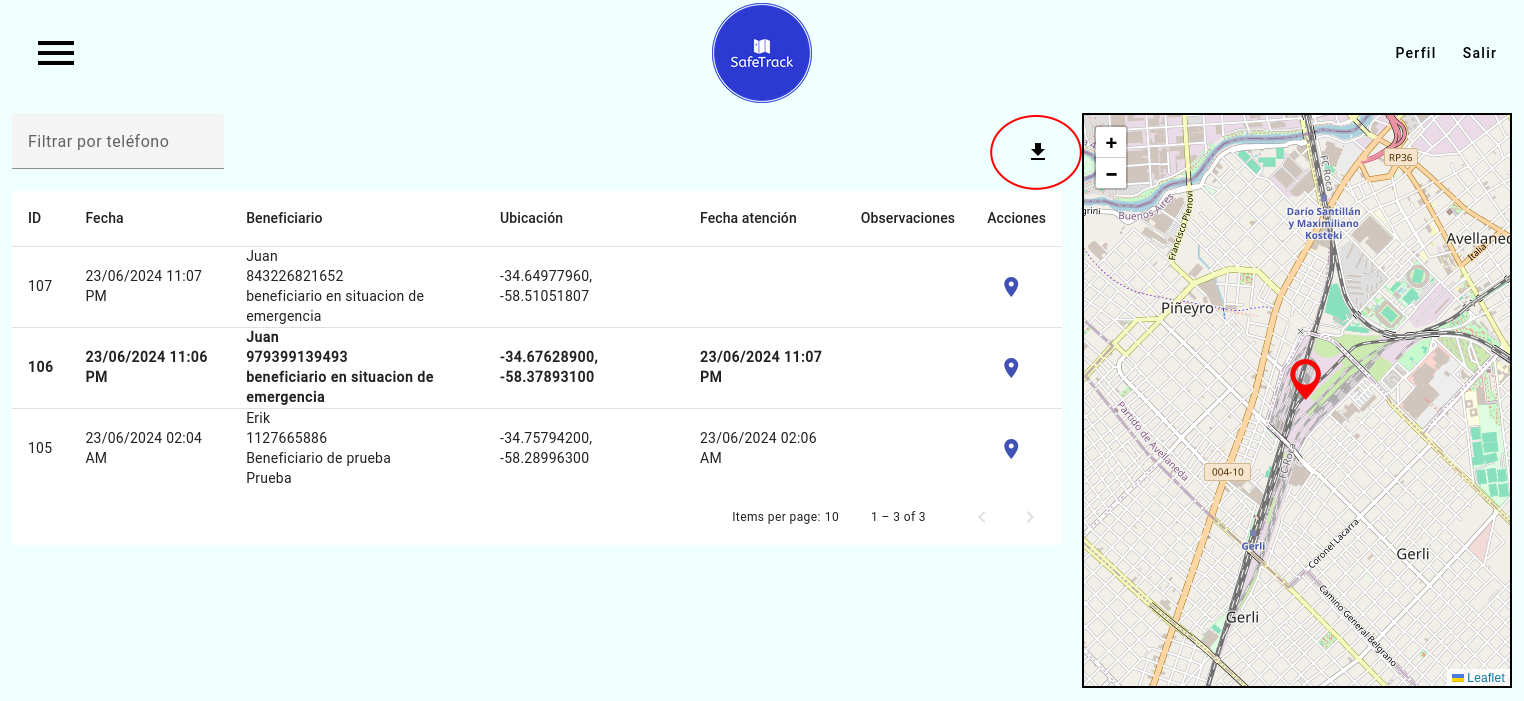
\includegraphics[width=1\linewidth]{./Figures/listado-alertas.png}
  	\captionof{figure}{Listado histórico de alertas y botón de exportación.}
  	\label{fig:frontend:alertas}
\end{figure}

Todas las pruebas fueron realizadas tanto en el ambiente local de desarrollo como en el ambiente desplegado en Heroku, a excepción del envío de alertas desde Twilio debido a que se requería contar con una URL pública.

\section{Comparación con productos similares}

No se encuentra una solución que integre tanto el componente embebido como el sistema web de tal forma que pueda hacerse comparación uno a uno. Sin embargo, el trabajo desarrollado permite demostrar que:
\begin{itemize}
	\item Es factible desarrollar un prototipo de botón antipánico de bajo gasto energético, si se continuara el trabajo de optimización de consumo energético de algunos componentes, como es el caso del ESP32 y el regulador LM2596.
	\item Es posible contar con un número telefónico virtual al cual se le pueden enviar las alertas por SMS y hacer que este reenvíe los mensajes a otros sistemas.
	\item Se puede contar con una aplicación web básica para la recepción de alertas en tiempo real.
	\item Fue posible desarrollar un dispositivo de hardware con costos relativamente bajos y prestaciones superiores.
\end{itemize}

La tabla \ref{tab:comparativa} presenta una breve comparativa de puntos interesantes del dispositivo embebido contrastado contra los dos modelos de botón antipánico presentados en el capítulo 1 del documento.

\begin{table}[H]
	\centering
	\caption[Comparativa de dispositivos embebidos.]{Comparativa de dispositivos embebidos.}
	\begin{tabular}{l c c c c}    
		\toprule
		\textbf{Modelo} & \textbf{\makecell{Duración \\ de batería}} & \textbf{\makecell{Tiempo para \\ conexión GSM}} & \textbf{\makecell{Tiempo para \\ conexión GPS}} & \textbf{\makecell{Precisión \\ GPS \textit{indoor}}} \\
		\midrule
		TK102B & Buena & Bueno & Medio & Medio \\ 
		LK109 & Mala & Bueno & Malo & Malo \\
		\makecell[l]{Desarrollo \\ propio} & Media & Bueno & Bueno & Muy bueno \\		
		\bottomrule
		\hline
	\end{tabular}
	\label{tab:comparativa}
\end{table}

En relación a las capacidades de las antenas, se observó una mejoría respecto a otros modelos existentes. Respecto a la duración de la batería, se concluye que también podría ser mejorable con baterías de mayor capacidad, aunque esto implicaría un aumento en el costo del dispositivo.


